%=========================================================================
%  Simulacion de Sistemas (72.25) - Trabajo Practico Nro. 5, Problema 2
%  Evacuacion con esquema hibrido EDMD + TSDMD. 13 minutos.
%  Preambulo (hasta "DATOS DEL GRUPO") copiado tal cual del TP4. Sigue
%  GuiaPresentaciones (guia X.Y) y las devoluciones del TP3 y del TP4.
%=========================================================================
\documentclass[11pt,aspectratio=169]{beamer}

%------------------------- VERSION ORAL / ENTREGA (guia 2.4.8) ----------
% Entrega en campus: \vivofalse -> fotograma fijo + link a YouTube debajo.
% Exposicion en vivo: \vivotrue -> animaciones con el paquete animate (PDFs de
% fotogramas en figuras/anim_lite/; se reproducen SOLO en Adobe Acrobat Reader;
% en otros visores se ve el primer fotograma). NUNCA entregar este pdf.
\newif\ifvivo
\vivotrue

%------------------------- TEMA (guia 1.12: miniframes) -----------------
\usetheme{Berlin}
\setbeamertemplate{itemize items}[square]
\setbeamertemplate{navigation symbols}{}
\setbeamertemplate{section in toc}{\inserttocsection}   % guia 1.13: sin numerar
\setbeamercovered{invisible}

% Titulo y subtitulo CENTRADOS dentro de la barra azul.
\setbeamertemplate{frametitle}[default][center]

\setbeamersize{text margin left=1.0cm, text margin right=1.0cm}

% Pie: SOLO el numero de diapositiva (guia 1.2). Correccion TP3: no repetir
% integrantes ni numero de grupo en todas las diapositivas.
\setbeamertemplate{footline}{%
  \leavevmode\hfill
  {\usebeamerfont{page number in head/foot}%
   \usebeamercolor[fg]{structure}\insertframenumber}%
  \hspace*{0.45cm}\vskip0.22cm}

%------------------------- PAQUETES -------------------------------------
\usepackage[utf8]{inputenc}
\usepackage[T1]{fontenc}
% En Overleaf existen ambos; el IfFileExists es solo para que compile
% tambien en distribuciones minimas.
\IfFileExists{spanish.ldf}
  {\usepackage[spanish,es-noshorthands]{babel}}
  {\usepackage[main=spanish,provide=*]{babel}}
\IfFileExists{lmodern.sty}{\usepackage{lmodern}}{}
\usepackage{amsmath,amssymb}
\usepackage{graphicx}
\usepackage{booktabs}
\usepackage{algpseudocode}
\usepackage{tikz}
\usetikzlibrary{arrows.meta,positioning,calc,shapes.multipart,shadows}
\ifvivo\usepackage{animate}\fi

\graphicspath{{figuras/}}

% Links de YouTube: con la letra del texto (mas angosta que la monoespaciada) y sin
% cortar despues de "https:" (asi quedaba el link de N = 50).
\usepackage{url}
\urlstyle{same}
\def\UrlBigBreaks{}

% Pseudocodigo en castellano
\algrenewcommand\algorithmicfor{\textbf{para}}
\algrenewcommand\algorithmicdo{\textbf{hacer}}
\algrenewcommand\algorithmicif{\textbf{si}}
\algrenewcommand\algorithmicthen{\textbf{entonces}}
\algrenewcommand\algorithmicend{\textbf{fin}}

%------------------------- NOTACION (guia 3.5) --------------------------
\newcommand{\vect}[1]{\mathbf{#1}}          % vector: negrita sin italica
\newcommand{\un}[1]{\,\mathrm{#1}}          % unidad: recta
\newcommand{\sci}[2]{#1\times 10^{#2}}      % guia 1.9: potencias de 10
\newcommand{\dt}{\Delta t}
% Correccion TP3 (D26): una sola notacion para el tiempo caracteristico.
\newcommand{\tnov}{\langle t_{90}\rangle}
\newcommand{\tcien}{\langle t_{100}\rangle}
\newcommand{\kT}{k_BT}
\newcommand{\ecmE}{\mathrm{ECM}_E}           % observable de 2.1 a)

% PENDIENTE: valor o conclusion a completar con los resultados.
% Buscar "\pend" antes de entregar: no debe quedar ninguno.
% Guia 1.10: los valores con error van con las cifras significativas del error.
\newcommand{\pend}[1]{\textcolor{red}{\textbf{[#1]}}}

%------------------------- BLOQUE DE CONTENIDO CENTRADO -----------------
% Bloque centrado de ancho fijo. Soporta columns y formulas en display.
% Ajustar el ancho con el argumento opcional: \begin{cuerpo}[0.73\textwidth]
\newenvironment{cuerpo}[1][0.88\textwidth]{%
  \par\vspace{0.2em}\begin{center}\begin{minipage}{#1}}%
  {\end{minipage}\end{center}}

% Vineta cuadrada del tema para usar en renglones centrados (fuera de itemize).
\newcommand{\vineta}{\raisebox{0.2ex}{\textcolor{structure.fg}{\rule{0.42em}{0.42em}}}}

\newcommand{\cajatitulo}[1]{%
  \begin{center}%
  \begin{minipage}{0.84\textwidth}%
    \begin{beamercolorbox}[wd=\linewidth,sep=14pt,center]{title}
      \usebeamerfont{title}#1
    \end{beamercolorbox}%
  \end{minipage}%
  \end{center}}

%------------------------- FIGURAS (guia 1.7 y 1.8) ---------------------
% Guia 1.7: las figuras NO llevan titulo adentro ni caption debajo; las
% condiciones de la corrida van en el panel al costado.
% Guia 1.8 / correccion TP3: fuentes de la figura >= tamano del texto.
% Si el archivo no existe se dibuja un recuadro gris con la ruta esperada.
\newcommand{\marcador}[3]{%
  \begin{tikzpicture}
    \node[draw=gray,dashed,thick,fill=gray!8,inner sep=0pt,
          minimum width=#1,minimum height=#2,
          align=center,text=gray!60,font=\scriptsize\ttfamily]
          {figuras/\detokenize{#3}};
  \end{tikzpicture}}

% Figura con panel lateral de parametros (columna de ~0.68\textwidth)
\newcommand{\figres}[1]{%
  \IfFileExists{figuras/#1}%
    {\includegraphics[width=\linewidth,height=0.68\textheight,keepaspectratio]{figuras/#1}}%
    {\marcador{0.95\linewidth}{0.64\textheight}{#1}}}

% Fotograma (cuadrado) de una animacion
\newcommand{\fotograma}[1]{%
  \IfFileExists{figuras/#1}%
    {\includegraphics[width=\linewidth,height=0.50\textheight,keepaspectratio]{figuras/#1}}%
    {\marcador{0.48\textheight}{0.48\textheight}{#1}}}

% Animacion (guia 2.4.8; correccion TP3: maximo dos por diapositiva):
%   \figanim{fotograma.png}{video.mp4}{link}
% En el pdf de entrega: fotograma fijo y DEBAJO el link explicito.
% En vivo (\vivotrue): animacion en loop desde figuras/anim_lite/#2.pdf (5 fps).
\newcommand{\figanim}[3]{%
  \ifvivo
    \animategraphics[autoplay,loop,height=0.50\textheight]{5}{figuras/anim_lite/#2}{}{}%
  \else
    \fotograma{#1}%
  \fi
  \par\vspace{0.3em}{\scriptsize\url{#3}}}

%------------------------- PANEL DE PARAMETROS --------------------------
% Correccion TP3: aca va el numero de realizaciones (M), NUNCA la semilla.
\newcommand{\panel}[1]{%
  \begin{block}{Parámetros}
    \scriptsize
    \begin{itemize}\setlength{\itemsep}{2.5pt}#1\end{itemize}
    \vspace{2pt}
  \end{block}}

% Leyenda de colores de las animaciones (va en el panel lateral)
\newcommand{\colores}{%
  \item \textcolor{blue!75}{$\blacksquare$}~fresca,
        \textcolor{red!80!black}{$\blacksquare$}~usada,
        $\blacksquare$~obstáculo}

%------------------------- SEPARADORES DE SECCION (guia 1.13) -----------
\AtBeginSection[]{%
  \begin{frame}
    \vfill
    \cajatitulo{\insertsectionhead}
    \vfill
  \end{frame}}

%------------------------- NOTACION DEL TP5 ----------------------------
% Correcciones TP4 (D12/D14): una letra para cada cosa. N es el numero de
% agentes; los que estan adentro son N_in. t es el tiempo simulado; el tiempo
% de ejecucion es T_ej (tau ya es la relajacion del SFM).
\algrenewcommand\algorithmicwhile{\textbf{mientras}}
\algrenewcommand\algorithmicelse{\textbf{si no}}
\newcommand{\Nin}{N_{\mathrm{in}}}
\newcommand{\NTS}{N_{\mathrm{TS}}}
\newcommand{\fTS}{f_{\mathrm{TS}}}
\newcommand{\fTSm}{\bar{f}_{\mathrm{TS}}}
\newcommand{\tevac}{t_{\mathrm{evac}}}
\newcommand{\Tej}{T_{\mathrm{ej}}}
\newcommand{\Rs}{R_s}
\newcommand{\vd}{v_d}
\newcommand{\ed}{\hat{\vect{e}}}
% Leyenda de colores de las animaciones del TP5 (Figura 1 del enunciado)
\newcommand{\coloresTP}{%
  \item \textcolor{blue!75}{$\blacksquare$}~EDMD,
        \textcolor{red!80!black}{$\blacksquare$}~TSDMD}

%------------------------- DATOS DEL GRUPO ------------------------------
\title[Evacuación con Esquema Híbrido]{Trabajo Práctico N.º 5:\\ Evacuación con Esquema Híbrido EDMD + TSDMD}
\author[N. Canzonieri, L. Díaz Varela, F. Viera]{Canzonieri, Nicolás \and Díaz Varela, Lola \and Viera, Federico}
\date{2026 2C}

\begin{document}

\begin{frame}
  \vfill
  \cajatitulo{Trabajo Práctico N.º 5:\\[2pt]
    Dinámica Peatonal: Evacuación con\\ Esquema Híbrido Event Driven + Time Step Driven\par
    \vskip8pt
    {\normalsize 72.25 --- Simulación de Sistemas}}

  \vskip2.2em
  \begin{center}
    {\large\textbf{2026 2C --- Grupo 9}}\par
    \vskip1.0em
    \vineta~Canzonieri, Nicolás (63501)\par
    \vskip0.45em
    \vineta~Díaz Varela, Lola (62792)\par
    \vskip0.45em
    \vineta~Viera, Federico (62022)\par
  \end{center}
  \vfill
\end{frame}

%=========================================================================
\section{Introducción}
%=========================================================================
% Guia 2.1: maximo 3 diapositivas, modelo GENERAL (sin N, L, d ni radios;
% correccion TP3 D4-D7). Consideracion (i) de la catedra: ademas, como choca
% EDMD y como recupera v_d (manda el enunciado sobre la guia).

\begin{frame}
  \frametitle{Sistema Real}

  \vfill
  \begin{cuerpo}[0.80\textwidth]
    \begin{itemize}\setlength{\itemsep}{0.8em}
      \item Peatones que evacúan una sala por una salida angosta, cada uno con una velocidad deseada.
      \item Lejos de la salida: vuelo libre y choques aislados.
      \item Cerca de la salida: cuello de botella y contacto permanente.
    \end{itemize}
  \end{cuerpo}
  \vfill
\end{frame}

\begin{frame}
  \frametitle{Fundamentos}
  \framesubtitle{Social Force Model sin fuerza social}

  \vfill
  \begin{cuerpo}[0.90\textwidth]
    \[
      m_i\frac{d\vect{v}_i}{dt}=
      \underbrace{m_i\,\frac{\vd\,\ed_i-\vect{v}_i}{\tau}}_{\text{deseo}}
      +\sum_{j:\ \xi_{ij}>0}\Big[-k_n\,\xi_{ij}\,\hat{\vect{e}}^{\,n}_{ij}
      -k_t\,\xi_{ij}\,\big(\Delta\vect{v}_{ij}\cdot\hat{\vect{e}}^{\,t}_{ij}\big)\,\hat{\vect{e}}^{\,t}_{ij}\Big]
      +\vect{F}^{\,\mathrm{pared}}_i
    \]
    \vspace{0.3em}
    \[
      \xi_{ij}=R_i+R_j-\left|\vect{r}_j-\vect{r}_i\right|,
      \qquad
      \hat{\vect{e}}^{\,n}_{ij}=\frac{\vect{r}_j-\vect{r}_i}{\left|\vect{r}_j-\vect{r}_i\right|},
      \qquad
      \ed_i=\frac{\vect{r}^{\,\mathrm{target}}_i-\vect{r}_i}{\left|\vect{r}^{\,\mathrm{target}}_i-\vect{r}_i\right|}
    \]
    \vspace{0.3em}
    {\small $\vd$: velocidad deseada;\quad $\tau$: tiempo de relajación;\quad $R_i$: radio;\quad
    $k_n$, $k_t$: constantes normal y tangencial.\par
    La pared actúa como un agente quieto en el punto más cercano del segmento.}
  \end{cuerpo}
  \vfill
\end{frame}

\begin{frame}
  \frametitle{Fundamentos}
  \framesubtitle{Event Driven: colisión instantánea}

  \vfill
  \begin{cuerpo}[0.80\textwidth]
    Entre eventos, cada agente se mueve en línea recta a velocidad constante.
    Choque con restitución $e$:
    \[
      \vect{v}_i'=\vect{v}_i+\frac{J}{m_i}\,\hat{\vect{e}}^{\,n}_{ij},
      \qquad
      \vect{v}_j'=\vect{v}_j-\frac{J}{m_j}\,\hat{\vect{e}}^{\,n}_{ij}
    \]
    \[
      J=(1+e)\,\frac{m_im_j}{m_i+m_j}\,\big(\Delta\vect{v}_{ij}\cdot\hat{\vect{e}}^{\,n}_{ij}\big)
    \]
    {\small La componente normal relativa sale con $e$ veces la de entrada; la tangencial no cambia.}
  \end{cuerpo}
  \vfill
\end{frame}

\begin{frame}
  \frametitle{Fundamentos}
  \framesubtitle{Event Driven: recuperación de la velocidad deseada}

  \vfill
  \begin{cuerpo}[0.80\textwidth]
    Sin contactos, la fuerza de deseo tiene solución exacta:
    \[
      \vect{v}(t+\Delta\tau)=\vd\,\ed+\big[\vect{v}(t)-\vd\,\ed\big]\,e^{-\Delta\tau/\tau}
    \]
    {\small Se aplica en eventos fantasma; entre ellos la velocidad queda fija.}
  \end{cuerpo}
  \vfill
\end{frame}

%=========================================================================
\section{Implementación}
%=========================================================================
% Guia 2.2: solo el motor. Correccion TP4 (D7): el UML NO tiene observables.
% Enunciado (a): mas tiempo que lo habitual para el esquema hibrido.

\begin{frame}
  \frametitle{Arquitectura del Motor}

  \vfill
  \begin{center}
  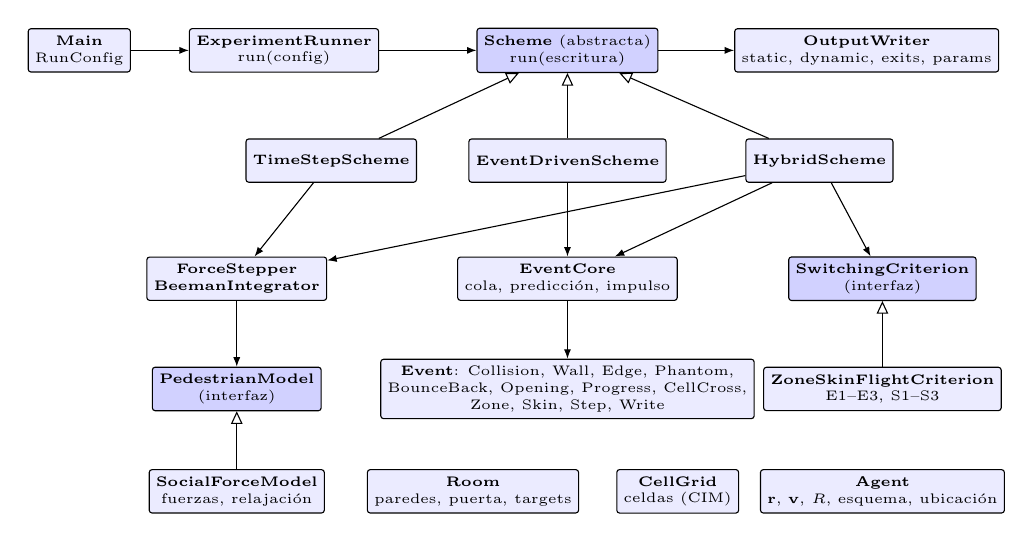
\begin{tikzpicture}[
      cls/.style={draw,rounded corners=1pt,fill=blue!8,font=\tiny,align=center,
                  inner sep=2.5pt,minimum height=0.55cm},
      abs/.style={cls,fill=blue!18},
      inh/.style={-{Triangle[open,length=1.6mm]},thin},
      use/.style={-{Latex[length=1.2mm]},thin}]
    \node[cls] (main) at (0,0) {\textbf{Main}\\RunConfig};
    \node[cls] (runner) at (2.6,0) {\textbf{ExperimentRunner}\\run(config)};
    \node[abs] (scheme) at (6.2,0) {\textbf{Scheme} (abstracta)\\run(escritura)};
    \node[cls] (writer) at (10.0,0) {\textbf{OutputWriter}\\static, dynamic, exits, params};
    \node[cls] (ts) at (3.2,-1.4) {\textbf{TimeStepScheme}};
    \node[cls] (ed) at (6.2,-1.4) {\textbf{EventDrivenScheme}};
    \node[cls] (hy) at (9.4,-1.4) {\textbf{HybridScheme}};
    \node[cls] (stepper) at (2.0,-2.9) {\textbf{ForceStepper}\\\textbf{BeemanIntegrator}};
    \node[cls] (core) at (6.2,-2.9) {\textbf{EventCore}\\cola, predicción, impulso};
    \node[cls] (event) at (6.2,-4.3) {\textbf{Event}: Collision, Wall, Edge, Phantom,\\BounceBack, Opening, Progress, CellCross,\\Zone, Skin, Step, Write};
    \node[abs] (crit) at (10.2,-2.9) {\textbf{SwitchingCriterion}\\(interfaz)};
    \node[cls] (zsf) at (10.2,-4.3) {\textbf{ZoneSkinFlightCriterion}\\E1--E3, S1--S3};
    \node[abs] (model) at (2.0,-4.3) {\textbf{PedestrianModel}\\(interfaz)};
    \node[cls] (sfm) at (2.0,-5.6) {\textbf{SocialForceModel}\\fuerzas, relajación};
    \node[cls] (room) at (5.0,-5.6) {\textbf{Room}\\paredes, puerta, targets};
    \node[cls] (grid) at (7.6,-5.6) {\textbf{CellGrid}\\celdas (CIM)};
    \node[cls] (agent) at (10.2,-5.6) {\textbf{Agent}\\$\vect{r}$, $\vect{v}$, $R$, esquema, ubicación};
    \draw[use] (main) -- (runner);
    \draw[use] (runner) -- (scheme);
    \draw[use] (scheme) -- (writer);
    \draw[inh] (ts) -- (scheme);
    \draw[inh] (ed) -- (scheme);
    \draw[inh] (hy) -- (scheme);
    \draw[use] (ts) -- (stepper);
    \draw[use] (ed) -- (core);
    \draw[use] (hy) -- (core);
    \draw[use] (hy) -- (stepper);
    \draw[use] (hy) -- (crit);
    \draw[use] (core) -- (event);
    \draw[inh] (zsf) -- (crit);
    \draw[use] (stepper) -- (model);
    \draw[inh] (sfm) -- (model);
  \end{tikzpicture}
  \end{center}
  \vfill
\end{frame}

%------------------------------------------------------------------- TSDMD
\begin{frame}
  \frametitle{TSDMD Puro}
  \framesubtitle{Integrador: Beeman predictor-corrector}

  \vfill
  \begin{cuerpo}[0.80\textwidth]
    \small
    \[
      \vect{r}(t+\dt)=\vect{r}+\vect{v}\dt+\tfrac{2}{3}\vect{a}\dt^2-\tfrac{1}{6}\vect{a}(t-\dt)\dt^2
    \]
    \[
      \vect{v}^{\,p}(t+\dt)=\vect{v}+\tfrac{3}{2}\vect{a}\dt-\tfrac{1}{2}\vect{a}(t-\dt)\dt
    \]
    \[
      \vect{a}(t+\dt)=\vect{F}\big(\vect{r}(t+\dt),\vect{v}^{\,p}(t+\dt)\big)/m
    \]
    \[
      \vect{v}(t+\dt)=\vect{v}+\tfrac{1}{3}\vect{a}(t+\dt)\dt+\tfrac{5}{6}\vect{a}\dt-\tfrac{1}{6}\vect{a}(t-\dt)\dt
    \]
    Las fuerzas del SFM dependen de $\vect{v}$: se evalúan con la velocidad predicha $\vect{v}^{\,p}$.
  \end{cuerpo}
  \vfill
\end{frame}

\begin{frame}
  \frametitle{TSDMD Puro}
  \framesubtitle{Algoritmo implementado}

  \vfill
  \begin{cuerpo}[0.70\textwidth]
    \hrule height 0.4pt\vspace{3pt}
    {\small
    \begin{algorithmic}[1]
      \While{queden agentes}
        \State Armar celdas (CIM)
        \State Beeman: predecir $\vect{r}$, $\vect{v}^{\,p}$
        \State Fuerzas SFM entre vecinos y con paredes
        \State Corregir $\vect{v}$
        \State Cambio de target, cruce de puerta, retiro
        \If{$n \bmod k=0$} \Comment{$\dt_2=k\,\dt$}
          \State Escribir $t$ y el estado de cada agente
        \EndIf
      \EndWhile
    \end{algorithmic}}
    \vspace{3pt}\hrule height 0.4pt
  \end{cuerpo}
  \vfill
\end{frame}

%-------------------------------------------------------------------- EDMD
\begin{frame}
  \frametitle{EDMD Puro}
  \framesubtitle{Predicción de choques}

  \vfill
  \begin{center}
    \textbf{Tiempo de choque entre dos agentes}
    \[
      t_c=-\frac{\Delta\vect{v}\cdot\Delta\vect{r}+\sqrt{d}}{\Delta\vect{v}\cdot\Delta\vect{v}},
      \qquad
      d=(\Delta\vect{v}\cdot\Delta\vect{r})^2-|\Delta\vect{v}|^2\big(|\Delta\vect{r}|^2-\sigma^2\big)
    \]
    {\small $\sigma=R_i+R_j$. Los bordes de la puerta son discos quietos de radio 0.}
  \end{center}
  \vfill
\end{frame}

\begin{frame}
  \frametitle{EDMD Puro}
  \framesubtitle{Restitución sacada del SFM}

  \vfill
  \begin{center}
    \textbf{Choque frontal blando}
    \[
      \ddot\xi+\frac{\dot\xi}{\tau}+\omega^2\xi=0,
      \qquad
      \omega^2=k_n\,\frac{m_i+m_j}{m_im_j}
      \qquad\Rightarrow\qquad
      e=e^{-\pi/(2\tau\omega)}
    \]
    \vspace{0.8em}
    \textbf{Piso de separación}
    \[
      v_n'=\max(e\,v_n,\ v_{\mathrm{sep}})
    \]
    {\small Evita infinitos choques en tiempo finito.}
  \end{center}
  \vfill
\end{frame}

\begin{frame}
  \frametitle{EDMD Puro}
  \framesubtitle{Eventos fantasma}

  \vfill
  \begin{cuerpo}[0.76\textwidth]
    \[
      \Delta\tau_i=\frac{R_i}{\max\left(|\vect{v}_i|,\ \vd\right)}
    \]
    \begin{itemize}\setlength{\itemsep}{0.6em}
      \item Lo que tarda el agente en recorrer su radio.
      \item Un choque no reinicia el fantasma pendiente.
      \item Si $|\vect{v}_i-\vd\ed_i|<0.01\,\vd$: $\vect{v}_i=\vd\ed_i$ y se cortan los fantasmas.
    \end{itemize}
  \end{cuerpo}
  \vfill
\end{frame}

\begin{frame}
  \frametitle{EDMD Puro}
  \framesubtitle{Eventos propios}

  \vfill
  \begin{center}
    \scriptsize
    \renewcommand{\arraystretch}{1.5}
    \begin{tabular}{@{}l p{0.34\textwidth} p{0.34\textwidth}@{}}
      \toprule
      \textbf{Evento} & \textbf{Cuándo ocurre} & \textbf{Qué hace}\\
      \midrule
      Fantasma & Cada $\Delta\tau_i$, mientras $\vect{v}_i\neq\vd\ed_i$ & Aplica la solución exacta del deseo\\
      Bounce back & Cuando el fantasma dejaría $|\vect{v}_i-\vd\ed_i|<0.01\,\vd$ & Fija $\vect{v}_i=\vd\ed_i$ y corta los fantasmas\\
      Progreso & Cruce de $y=R_i$, $y=0$ o $y=-1\un{m}$ & Cambio de target, cruce de la puerta o retiro\\
      Vano & Entra de costado al vano de la puerta & Recalcula su target\\
      Cruce de celda & Sale de su celda de la grilla & Actualiza el CIM y predice contra los vecinos nuevos\\
      Escritura & Cada $\dt_2$ & Avanza a todos los agentes y escribe el estado\\
      \bottomrule
    \end{tabular}

    \vspace{1em}
    {\scriptsize Además, los choques clásicos: agente--agente, agente--pared y agente--borde de la puerta.}
  \end{center}
  \vfill
\end{frame}

\begin{frame}
  \frametitle{EDMD Puro}
  \framesubtitle{Algoritmo implementado}

  \vfill
  \begin{cuerpo}[0.78\textwidth]
    \hrule height 0.4pt\vspace{3pt}
    {\small
    \begin{algorithmic}[1]
      \State Predecir los eventos de cada agente
      \While{queden agentes}
        \State $ev\gets$ próximo evento válido de la cola
        \State Avanzar solo los agentes de $ev$
        \State Aplicar $ev$ \Comment{choque, fantasma, celda, escritura\dots}
        \State Contador de esos agentes $+1$ \Comment{invalida}
        \State Predecir sus eventos contra vecinos (CIM), paredes y bordes
      \EndWhile
    \end{algorithmic}}
    \vspace{3pt}\hrule height 0.4pt
  \end{cuerpo}
  \vfill
\end{frame}

%----------------------------------------------------------------- HIBRIDO
% Profesor (2026-11-13): una diapositiva por condicion y cada variable
% definida donde aparece por primera vez; los valores van en Simulaciones.
\begin{frame}
  \frametitle{Esquema Híbrido}
  \framesubtitle{De EDMD a TSDMD, alcanza con una: E1 Zona}

  \vfill
  \begin{columns}[c]
    \begin{column}{0.56\textwidth}
      \centering
      \[
        r_i\le\Rs
      \]
      \vspace{0.6em}
      \textbf{Detecta:} cercanía a la puerta, donde se forma la multitud.\par
      \vspace{1.2em}
      {\small $r_i$: distancia del agente al centro de la puerta;\quad
      $\Rs$: radio de la zona TSDMD.\par
      Es un evento con tiempo exacto: la cuadrática del choque con $\sigma=\Rs$.\par
      Animación: 6 agentes, $\Rs=3\un{m}$, sin E3.}
    \end{column}
    \begin{column}{0.40\textwidth}
      \centering
      \figanim{criterios/anim_criterio_E1.png}{anim_criterio_E1}{\pend{link de YouTube}}
    \end{column}
  \end{columns}
  \vfill
\end{frame}

\begin{frame}
  \frametitle{Esquema Híbrido}
  \framesubtitle{De EDMD a TSDMD, alcanza con una: E2 Contagio}

  \vfill
  \begin{columns}[c]
    \begin{column}{0.56\textwidth}
      \centering
      \[
        g_{ij}\le\delta_{\mathrm{in}}\quad\text{con algún } j \text{ en TSDMD}
      \]
      \[
        g_{ij}=|\vect{r}_j-\vect{r}_i|-(R_i+R_j)
      \]
      \vspace{0.6em}
      \textbf{Detecta:} un agente duro a punto de chocar con uno blando.\par
      \vspace{1.2em}
      {\small $g_{ij}$: separación entre bordes;\quad $\delta_{\mathrm{in}}$: piel de entrada.\par
      En cadena: el que pasa a TSDMD contagia a sus vecinos EDMD.\par
      Animación: atasco en la zona ($\Rs=1.5\un{m}$), sin E3: los de atrás pasan afuera de ella.}
    \end{column}
    \begin{column}{0.40\textwidth}
      \centering
      \figanim{criterios/anim_criterio_E2.png}{anim_criterio_E2}{\pend{link de YouTube}}
    \end{column}
  \end{columns}
  \vfill
\end{frame}

\begin{frame}
  \frametitle{Esquema Híbrido}
  \framesubtitle{Chequeo de piel (E2)}

  \vfill
  \begin{cuerpo}[0.80\textwidth]
    Cada agente EDMD agenda su próximo chequeo en
    \[
      t+\frac{g_{\min}-\delta_{\mathrm{in}}}{|\vect{v}_i|+v_{\max}}
    \]
    \begin{itemize}\setlength{\itemsep}{0.6em}
      \item $g_{\min}$: separación al TSDMD más cercano; $v_{\max}$: cota de la velocidad de los TSDMD.
      \item $\delta_{\mathrm{in}}\ge 2\,v_{\max}\dt$: no se pierden contactos.
      \item Si un TSDMD supera $v_{\max}$, el motor corta con error.
    \end{itemize}
  \end{cuerpo}
  \vfill
\end{frame}

\begin{frame}
  \frametitle{Esquema Híbrido}
  \framesubtitle{De EDMD a TSDMD, alcanza con una: E3 Vuelo}

  \vfill
  \begin{columns}[c]
    \begin{column}{0.56\textwidth}
      \centering
      \[
        t_{\mathrm{vuelo},i}<t_s,
        \qquad
        t_s=\frac{\pi}{\omega}
      \]
      \vspace{0.6em}
      \textbf{Detecta:} choques más seguidos que lo que dura un choque blando.\par
      \vspace{1.2em}
      {\small $t_{\mathrm{vuelo},i}$: tiempo entre dos choques seguidos del agente;\quad
      $t_s$: duración de un rebote blando del SFM.\par
      Se evalúa en cada choque.\par
      Animación: $\Rs=0$, sin zona: los primeros pasan por E3; después, contagio.}
    \end{column}
    \begin{column}{0.40\textwidth}
      \centering
      \figanim{criterios/anim_criterio_E3.png}{anim_criterio_E3}{\pend{link de YouTube}}
    \end{column}
  \end{columns}
  \vfill
\end{frame}

\begin{frame}
  \frametitle{Esquema Híbrido}
  \framesubtitle{De TSDMD a EDMD, tienen que cumplirse las tres: S1 Zona}

  \vfill
  \begin{center}
    \[
      r_i\ge\Rs+h
    \]
    \vspace{0.6em}
    \textbf{Detecta:} el agente salió de la zona alrededor de la puerta.\par
    \vspace{1.2em}
    {\small $h$: histéresis, para que un agente en el borde de la zona no cambie de esquema en cada paso.}
  \end{center}
  \vfill
\end{frame}

\begin{frame}
  \frametitle{Esquema Híbrido}
  \framesubtitle{De TSDMD a EDMD, tienen que cumplirse las tres: S2 Piel}

  \vfill
  \begin{center}
    \[
      g_{ij}\ge\delta_{\mathrm{out}}\quad\text{con todo } j,\ \text{sin tocar paredes},
      \qquad
      \delta_{\mathrm{out}}>\delta_{\mathrm{in}}
    \]
    \vspace{0.6em}
    \textbf{Detecta:} el agente quedó sin contactos; el choque instantáneo vuelve a valer.\par
    \vspace{1.2em}
    {\small $\delta_{\mathrm{out}}$: piel de salida.\par
    Se chequea en cada paso de TSDMD, solo si ya se cumplen S1 y S3. Con celdas de lado
    $\ge 2R_{\max}+\delta_{\mathrm{out}}$, alcanza con mirar las $3\times3$ celdas vecinas.}
  \end{center}
  \vfill
\end{frame}

\begin{frame}
  \frametitle{Esquema Híbrido}
  \framesubtitle{De TSDMD a EDMD, tienen que cumplirse las tres: S3 Velocidad}

  \vfill
  \begin{center}
    \[
      |\vect{v}_i-\vd\ed_i|\le\varepsilon\,\vd
    \]
    \vspace{0.6em}
    \textbf{Detecta:} el agente recuperó la velocidad deseada: vuelve al vuelo libre.\par
    \vspace{1.2em}
    {\small $\varepsilon$: tolerancia relativa de velocidad.}
  \end{center}
  \vfill
\end{frame}

\begin{frame}
  \frametitle{Esquema Híbrido}
  \framesubtitle{Casos extremos}

  \vfill
  \begin{cuerpo}[0.80\textwidth]
    \begin{itemize}\setlength{\itemsep}{0.8em}
      \item $\Rs=0$ y $t_s=0$: nadie pasa a TSDMD $\Rightarrow$ \textbf{EDMD puro}.
      \item $\Rs\ge\sqrt{(L/2)^2+L^2}$, con $L$ el lado de la sala: todos en TSDMD desde $t=0$
            $\Rightarrow$ \textbf{TSDMD puro}.
      \item Los dos extremos reproducen bit a bit a los esquemas puros.
    \end{itemize}
  \end{cuerpo}
  \vfill
\end{frame}

\begin{frame}
  \frametitle{Esquema Híbrido}
  \framesubtitle{Sincronización}

  \vfill
  \begin{cuerpo}[0.84\textwidth]
    \begin{itemize}\setlength{\itemsep}{0.8em}
      \item El reloj global es la cola de eventos, como en EDMD puro.
      \item El paso de Beeman de los TSDMD es un evento más, en $n\,\dt$: solo existe mientras haya agentes
            en TSDMD. Sin ellos, el híbrido avanza de evento en evento.
      \item En el mismo instante: eventos de agentes, después el paso, después la escritura.
      \item Los cambios de esquema se aplican en el paso, con todos los agentes en el mismo instante.
      \item Fuerzas solo entre TSDMD: por E2, un EDMD pasa a TSDMD antes de tocar a uno.
      \item Sin superposiciones: a TSDMD se llega con $g>0$; a EDMD, con $g\ge\delta_{\mathrm{out}}$.
    \end{itemize}
  \end{cuerpo}
  \vfill
\end{frame}

% Para defender el costo y el radio: que se calcula y que no en cada paso, y que
% pasa con lo que se habia predicho hacia un agente que pasa a TSDMD.
\begin{frame}
  \frametitle{Esquema Híbrido}
  \framesubtitle{Qué se calcula en cada paso}

  \vfill
  \begin{cuerpo}[0.84\textwidth]
    \begin{itemize}\setlength{\itemsep}{0.8em}
      \item En cada paso, solo Beeman de los TSDMD: fuerzas entre TSDMD y celdas de los TSDMD.
      \item Los EDMD no se tocan: ni se mueven ni se les predicen choques nuevos. Su posición sale de la
            recta y se calcula en su próximo evento o en la escritura.
      \item Solo los EDMD vecinos de un TSDMD hacen chequeo de piel, en su horizonte seguro y no en cada paso.
      \item Costo: un paso cuesta según $\NTS$, no según $N$; los eventos, solo los de los EDMD.
    \end{itemize}
  \end{cuerpo}
  \vfill
\end{frame}

\begin{frame}
  \frametitle{Esquema Híbrido}
  \framesubtitle{Predicciones hacia un agente que pasa a TSDMD}

  \vfill
  \begin{cuerpo}[0.84\textwidth]
    \begin{itemize}\setlength{\itemsep}{0.8em}
      \item $j$ pasa a TSDMD: se invalidan todos los eventos predichos con $j$. Nunca se predice contra un TSDMD.
      \item Un EDMD $i$ que iba a chocar con $j$ conserva el resto de sus eventos: paredes, otros EDMD,
            fantasma, zona y piel.
      \item $i$ no puede tocar a $j$: el chequeo de piel lo pasa a TSDMD antes (E2).
      \item Si va hacia la puerta, además cruza $\Rs$ y pasa por E1, aunque no se acerque a $j$.
    \end{itemize}
    \vspace{0.6em}
    {\small El radio solo no alcanza: $j$ puede estar fuera de la zona, por contagio. La garantía la da E2.}
  \end{cuerpo}
  \vfill
\end{frame}

\begin{frame}
  \frametitle{Esquema Híbrido}
  \framesubtitle{Eventos propios}

  \vfill
  \begin{center}
    \scriptsize
    \renewcommand{\arraystretch}{1.5}
    \begin{tabular}{@{}l p{0.34\textwidth} p{0.34\textwidth}@{}}
      \toprule
      \textbf{Evento} & \textbf{Cuándo ocurre} & \textbf{Qué hace}\\
      \midrule
      Paso TSDMD & En $n\,\dt$, mientras haya agentes TSDMD o marcados & Un paso de Beeman de los TSDMD y los cambios de esquema\\
      Zona (E1) & $r_i=\Rs$: tiempo exacto, la cuadrática con $\sigma=\Rs$ & Marca al agente para pasar a TSDMD en el próximo paso\\
      Piel (E2) & $t+(g_{\min}-\delta_{\mathrm{in}})/(|\vect{v}_i|+v_{\max})$ & Si $g\le\delta_{\mathrm{in}}$ con un TSDMD, lo marca; si no, reagenda. No invalida sus otros eventos\\
      \bottomrule
    \end{tabular}

    \vspace{1em}
    {\scriptsize E3 no es un evento: se evalúa en cada choque.}
  \end{center}
  \vfill
\end{frame}

\begin{frame}
  \frametitle{Esquema Híbrido}
  \framesubtitle{Algoritmo implementado}

  \vfill
  \begin{cuerpo}[0.86\textwidth]
    \hrule height 0.4pt\vspace{3pt}
    {\footnotesize
    \begin{algorithmic}[1]
      \State Pasar a TSDMD a los agentes con $r_i\le\Rs$; predecir los eventos de los EDMD
      \State Agendar la escritura y, si hay TSDMD, el paso en $\dt$
      \While{queden agentes}
        \State $ev\gets$ próximo evento válido \Comment{agentes, paso, escritura}
        \If{$ev$ es de un agente}
          \State Como en EDMD; si E1, E2 o E3 $\to$ marcar y, si no hay, agendar paso
        \ElsIf{$ev$ es el paso en $n\,\dt$}
          \State Beeman de los TSDMD; target, puerta, retiro; verificar $|\vect{v}|\le v_{\max}$
          \State Marcados y vecinos a menos de $\delta_{\mathrm{in}}$ (E2) $\to$ TSDMD, en cadena
          \State Cumplen S1, S2 y S3 $\to$ EDMD; si quedan TSDMD, agendar paso en $(n+1)\,\dt$
        \Else
          \State Avanzar los EDMD y escribir el estado de cada agente
        \EndIf
      \EndWhile
    \end{algorithmic}}
    \vspace{3pt}\hrule height 0.4pt
  \end{cuerpo}
  \vfill
\end{frame}

%=========================================================================
\section{Simulaciones}
%=========================================================================
% Guia 2.3 y correccion TP3 (D13): esquema del sistema, parametros fijos y
% variables, observables definidos matematicamente, repeticiones.
% Correccion TP4 (D11): sin tabla de estudios. Consulta del TP4: dt, dt2 y el
% integrador son del METODO, no del sistema: van en una diapositiva aparte.

\begin{frame}
  \frametitle{Parámetros de Simulación}
  \framesubtitle{Esquema y parámetros fijos del sistema}

  \vfill
  \begin{columns}[c]
    \begin{column}{0.46\textwidth}
      \centering
      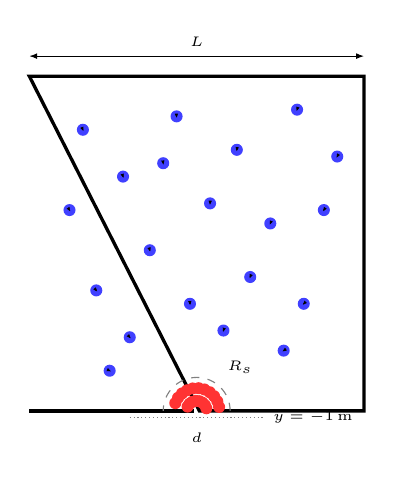
\begin{tikzpicture}[scale=0.085]
        % sala [0,L]^2 con la puerta en y = 0
        \draw[very thick] (0,0) -- (24.6,0);
        \draw[very thick] (25.4,0) -- (50,0) -- (50,50) -- (0,50) -- cycle;
        \draw[gray,densely dotted] (15,-1) -- (35,-1) node[right,font=\tiny,text=black]{$y=-1\un{m}$};
        \draw[dashed,gray] (30,0) arc (0:180:5);
        \node[font=\tiny] at (31.5,6.5) {$\Rs$};
        % agentes diluidos (EDMD)
        \foreach \x/\y in {8/42,14/35,22/44,31/39,40/45,44/30,36/28,27/31,18/24,10/18,
                           6/30,33/20,41/16,24/16,15/11,38/9,12/6,29/12,20/37,46/38}
          {\fill[blue!75] (\x,\y) circle (0.9);
           \draw[-{Latex[length=0.6mm]},thin] (\x,\y) -- ($(\x,\y)!0.3cm!(25,0)$);}
        % multitud en la puerta (TSDMD)
        \foreach \a in {15,35,...,165} {\fill[red!80] ($(25,0)+(\a:1.5)$) circle (0.9);}
        \foreach \a in {10,25,...,170} {\fill[red!80] ($(25,0)+(\a:3.4)$) circle (0.9);}
        % cotas
        \draw[{Latex[length=1mm]}-{Latex[length=1mm]}] (0,53) -- (50,53) node[midway,above,font=\tiny]{$L$};
        \node[below,font=\tiny] at (25,-1.8) {$d$};
      \end{tikzpicture}\par\vspace{0.2em}
      {\scriptsize \textcolor{blue!75}{$\blacksquare$}~EDMD\quad \textcolor{red!80}{$\blacksquare$}~TSDMD}
    \end{column}
    \begin{column}{0.50\textwidth}
      \centering
      \scriptsize
      \renewcommand{\arraystretch}{1.15}
      \begin{tabular}{@{}l@{\hspace{0.8em}}l@{\hspace{1.0em}}l@{}}
        \toprule
        \textbf{Símbolo} & \textbf{Valor} & \textbf{Descripción}\\
        \midrule
        $L$ & $50\un{m}$ & Lado de la sala\\
        $d$ & $0.8\un{m}$ & Ancho de la puerta\\
        $R_i$ & $U[0.18,\,0.25]\un{m}$ & Radio de cada agente\\
        $m$ & $80\un{kg}$ & Masa\\
        $\vd$ & $1.5\un{m/s}$ & Velocidad deseada; $\vect{v}(0)=\vd\ed$\\
        $\tau$ & $0.5\un{s}$ & Tiempo de relajación\\
        $k_n$ & $\sci{1.2}{5}\un{N/m}$ & Constante normal\\
        $k_t$ & $0$ & Sin fricción tangencial\\
        Target & $(L/2,\,R_i)$; $(L/2,-2\un{m})$ & Antes y después de la puerta\\
        \bottomrule
      \end{tabular}
    \end{column}
  \end{columns}
  \vfill
\end{frame}

\begin{frame}
  \frametitle{Parámetros de Simulación}
  \framesubtitle{Parámetros de los métodos}

  \vfill
  \begin{center}
    \scriptsize
    \renewcommand{\arraystretch}{1.2}
    \begin{tabular}{@{}l@{\hspace{1.0em}}l@{\hspace{1.0em}}l@{\hspace{1.0em}}l@{}}
      \toprule
      & \textbf{Símbolo} & \textbf{Valor} & \textbf{Descripción}\\
      \midrule
      Todos & $\dt_2$ & $\sci{5}{-1}\un{s}$ & Intervalo de escritura\\
      \midrule
      TSDMD & $\dt$ & $10^{-3}\un{s}$ & Paso temporal\\
      \midrule
      EDMD & $e$ & $0.94$; $0.92$ & Restitución entre agentes; con paredes\\
           & $v_{\mathrm{sep}}$ & $\sci{2}{-2}\un{m/s}$ & Piso de separación\\
      \midrule
      Híbrido & $t_s$ & $\sci{5.7}{-2}\un{s}$ & Tiempo de vuelo mínimo\\
              & $\delta_{\mathrm{in}}$; $\delta_{\mathrm{out}}$ & $\sci{5}{-2}\un{m}$; $\sci{2.5}{-1}\un{m}$ & Pieles de entrada y salida\\
              & $h$ & $1\un{m}$ & Histéresis de la zona\\
              & $\varepsilon$ & $\sci{5}{-2}$ & Tolerancia de velocidad\\
              & $v_{\max}$ & $5\un{m/s}$ ($8\un{m/s}$ en d) & Cota de velocidad\\
      \bottomrule
    \end{tabular}
  \end{center}
  \vfill
\end{frame}

\begin{frame}
  \frametitle{Parámetros de Simulación}
  \framesubtitle{Parámetros variables}

  \vfill
  \begin{center}
    \small
    \renewcommand{\arraystretch}{1.3}
    \begin{tabular}{@{}l l l@{}}
      \toprule
      \textbf{Símbolo} & \textbf{Ítems a--c} & \textbf{Ítem d}\\
      \midrule
      $N$ & $200$ & $100$ a $1000$\\
      $M$ & $10$ & $3$\\
      $\Rs$ & $0$ a $56\un{m}$, 10 valores & $5\un{m}$\\
      $L$ & $50\un{m}$ & $50\un{m}$ o $\sqrt{N/0.2}$\\
      $t_f$ & Salida del último agente, $\le 10^{3}\un{s}$ & Salida del último agente, $\le 1.5\un{s}\times N$\\
      \bottomrule
    \end{tabular}

    \vspace{0.9em}
    \scriptsize
    \begin{tabular}{@{}r@{\hspace{0.6em}}p{0.72\textwidth}@{}}
      \textbf{$M$:}      & realizaciones independientes por caso, las mismas en los tres esquemas\\
      \textbf{$t_f$:}    & tiempo final de simulación\\
      \textbf{Output:}   & $t$, $\vect{r}_i$, $\vect{v}_i$, esquema y ubicación de cada agente cada $\dt_2$;
                           instante en que cada agente cruza la puerta
    \end{tabular}
  \end{center}
  \vfill
\end{frame}

% Guia 2.3 y correccion TP2 (D15): un observable por diapositiva, poco texto
% (como en el TP4).
\begin{frame}
  \frametitle{Observables}
  \framesubtitle{Curva de población y tiempo de evacuación}

  \vfill
  \begin{center}
    \textbf{Agentes en la habitación}
    \[
      \Nin(t)=N-\#\{i:\ t_{\mathrm{puerta},i}\le t\}
    \]
    \vspace{1.2em}
    \textbf{Tiempo de evacuación}
    \[
      \tevac=\max_i\ t_{\mathrm{puerta},i}
    \]
  \end{center}
  \vfill
\end{frame}

\begin{frame}
  \frametitle{Observables}
  \framesubtitle{Fracción de agentes en TSDMD}

  \vfill
  \begin{center}
    \textbf{Fracción en TSDMD y su promedio temporal}
    \[
      \fTS(t)=\frac{\NTS(t)}{\Nin(t)},
      \qquad
      \fTSm=\frac{1}{K}\sum_{k=1}^{K}\fTS(t_k)
    \]
    {\small $t_k$: los $K$ instantes guardados con $\Nin>0$.}
    \vspace{1.2em}

    \textbf{Saltos entre esquemas}\par
    {\small Cambios de esquema de cada agente entre dos instantes guardados seguidos,
    en cada sentido.}
  \end{center}
  \vfill
\end{frame}

\begin{frame}
  \frametitle{Observables}
  \framesubtitle{Tiempo de ejecución y promedios}

  \vfill
  \begin{center}
    \textbf{Tiempo de ejecución $\Tej$}\par
    {\small Medido alrededor del loop del motor, una corrida por vez, después de corridas de calentamiento.}
    \vspace{1.2em}

    \textbf{Promedio sobre las $M_c$ realizaciones completas}
    \[
      \langle X\rangle=\frac{1}{M_c}\sum_{q=1}^{M_c}X^{(q)},
      \qquad
      \sigma_X=\sqrt{\frac{1}{M_c-1}\sum_{q=1}^{M_c}\left(X^{(q)}-\langle X\rangle\right)^2}
    \]
    {\small Una corrida trabada no tiene $\tevac$: se informa y el punto se marca con símbolo vacío.}
  \end{center}
  \vfill
\end{frame}

%=========================================================================
\section{Resultados}
%=========================================================================
% Guia 2.4: para cada input, animacion -> evolucion temporal -> input vs
% observable con barras de error. Primero la puesta a punto del metodo (dt).

\begin{frame}
  \frametitle{Elección del Paso Temporal}
  \framesubtitle{Observable: $\langle\tevac\rangle$ en función de $\dt$}

  \vfill
  \begin{columns}[c]
    \begin{column}{0.66\textwidth}
      \centering
      \figres{dt/evacuation_vs_dt.png}
    \end{column}
    \begin{column}{0.30\textwidth}
      \panel{\item TSDMD puro, $N=200$
             \item $M=10$
             \item Tolerancia: $\pm\sigma$ de $\dt=10^{-4}\un{s}$
             \item Todos los $\dt$ la cumplen; se usa el de los estudios previos}
    \end{column}
  \end{columns}
  \vfill
\end{frame}

%------------------------------------------------------------------------- a)
\begin{frame}
  \frametitle{Los Tres Esquemas}
  \framesubtitle{Animaciones: TSDMD puro y EDMD puro}

  \vfill
  \begin{columns}[c]
    \begin{column}{0.36\textwidth}
      \centering
      \figanim{a/anim_tsdmd.png}{anim_tsdmd}{\pend{link de YouTube}}
    \end{column}
    \begin{column}{0.36\textwidth}
      \centering
      \figanim{a/anim_edmd.png}{anim_edmd}{\pend{link de YouTube}}
    \end{column}
    \begin{column}{0.24\textwidth}
      \panel{\item $N=200$
             \item Una realización}
    \end{column}
  \end{columns}
  \vfill
\end{frame}

\begin{frame}
  \frametitle{Esquema Híbrido}
  \framesubtitle{Animación y fracción de agentes en cada esquema}

  \vfill
  \begin{columns}[c]
    \begin{column}{0.36\textwidth}
      \centering
      \figanim{a/anim_hibrido.png}{anim_hibrido}{\pend{link de YouTube}}
    \end{column}
    \begin{column}{0.44\textwidth}
      \centering
      \figres{a/fraction_vs_time.png}
    \end{column}
    \begin{column}{0.18\textwidth}
      \panel{\item $N=200$
             \item $\Rs=5\un{m}$
             \item Una realización}
    \end{column}
  \end{columns}
  \vfill
\end{frame}

\begin{frame}
  \frametitle{Esquema Híbrido}
  \framesubtitle{Observable: $\langle\fTS(t)\rangle$}

  \vfill
  \begin{columns}[c]
    \begin{column}{0.66\textwidth}
      \centering
      \figres{a/ts_fraction_mean_vs_time.png}
    \end{column}
    \begin{column}{0.30\textwidth}
      \panel{\item $N=200$, $\Rs=5\un{m}$
             \item $M=10$
             \item Promedio sobre las realizaciones con $\Nin>0$
             \item Saltos por corrida: $197\pm1$ de EDMD a TSDMD; ninguno de vuelta, mirando cada $\dt_2$}
    \end{column}
  \end{columns}
  \vfill
\end{frame}

%------------------------------------------------------------------------- b)
\begin{frame}
  \frametitle{Curvas de Población}
  \framesubtitle{Observable: $\langle\Nin(t)\rangle$ de los tres esquemas}

  \vfill
  \begin{columns}[c]
    \begin{column}{0.66\textwidth}
      \centering
      \figres{b/population_mean_vs_time.png}
    \end{column}
    \begin{column}{0.30\textwidth}
      \panel{\item $N=200$, $\Rs=5\un{m}$
             \item $M=10$, mismas en los tres
             \item Híbrido: 9 completas}
    \end{column}
  \end{columns}
  \vfill
\end{frame}

\begin{frame}
  \frametitle{Tiempo de Evacuación}
  \framesubtitle{Observable: $\langle\tevac\rangle$ de los tres esquemas}

  \vfill
  \begin{columns}[c]
    \begin{column}{0.62\textwidth}
      \centering
      \figres{b/evacuation_by_scheme.png}
    \end{column}
    \begin{column}{0.34\textwidth}
      \panel{\item $N=200$, $\Rs=5\un{m}$
             \item $M=10$
             \item Diferencia con TSDMD puro, en errores estándar: EDMD $6$; híbrido $0.9$}
    \end{column}
  \end{columns}
  \vfill
\end{frame}

%------------------------------------------------------------------------- c)
\begin{frame}
  \frametitle{Parámetro del Criterio de Pasaje}
  \framesubtitle{Animaciones: $\Rs=0$ y $\Rs=20\un{m}$}

  \vfill
  \begin{columns}[c]
    \begin{column}{0.36\textwidth}
      \centering
      \figanim{c/anim_hibrido_Rs0.png}{anim_hibrido_Rs0}{\pend{link de YouTube}}
    \end{column}
    \begin{column}{0.36\textwidth}
      \centering
      \figanim{c/anim_hibrido_Rs20.png}{anim_hibrido_Rs20}{\pend{link de YouTube}}
    \end{column}
    \begin{column}{0.24\textwidth}
      \panel{\item Híbrido, $N=200$
             \item Una realización}
    \end{column}
  \end{columns}
  \vfill
\end{frame}

\begin{frame}
  \frametitle{Parámetro del Criterio de Pasaje}
  \framesubtitle{Evolución: $\fTS(t)$ y su escalar $\fTSm$}

  \vfill
  \begin{columns}[c]
    \begin{column}{0.40\textwidth}
      \centering
      \figres{c/ts_fraction_vs_time.png}
    \end{column}
    \begin{column}{0.40\textwidth}
      \centering
      \figres{c/ts_fraction_vs_rs.png}
    \end{column}
    \begin{column}{0.18\textwidth}
      \panel{\item $N=200$
             \item Izquierda: una realización por $\Rs$
             \item Derecha: $M=10$}
    \end{column}
  \end{columns}
  \vfill
\end{frame}

\begin{frame}
  \frametitle{Tiempo de Ejecución}
  \framesubtitle{Observable: $\langle\Tej\rangle$ en función de $\Rs$}

  \vfill
  \begin{columns}[c]
    \begin{column}{0.66\textwidth}
      \centering
      \figres{c/wall_clock_vs_rs.png}
    \end{column}
    \begin{column}{0.30\textwidth}
      \panel{\item $N=200$, $M=10$
             \item $\dt_2=5\un{s}$}
    \end{column}
  \end{columns}
  \vfill
\end{frame}

% Profesor (2026-11-13): la banda de EDMD aplasta al hibrido contra TSDMD;
% la misma figura sin EDMD, con el eje ajustado.
\begin{frame}
  \frametitle{Tiempo de Ejecución}
  \framesubtitle{Observable: $\langle\Tej\rangle$ en función de $\Rs$, sin EDMD puro}

  \vfill
  \begin{columns}[c]
    \begin{column}{0.66\textwidth}
      \centering
      \figres{c/wall_clock_vs_rs_no_edmd.png}
    \end{column}
    \begin{column}{0.30\textwidth}
      \panel{\item $N=200$, $M=10$
             \item $\dt_2=5\un{s}$}
    \end{column}
  \end{columns}
  \vfill
\end{frame}

\begin{frame}
  \frametitle{Tiempo de Evacuación}
  \framesubtitle{Observable: $\langle\tevac\rangle$ en función de $\Rs$}

  \vfill
  \begin{columns}[c]
    \begin{column}{0.66\textwidth}
      \centering
      \figres{c/evacuation_vs_rs.png}
    \end{column}
    \begin{column}{0.30\textwidth}
      \panel{\item $N=200$, $M=10$}
    \end{column}
  \end{columns}
  \vfill
\end{frame}

%------------------------------------------------------------------------- d)
\begin{frame}
  \frametitle{Escalamiento con el Número de Agentes}
  \framesubtitle{Animaciones: $N=100$ y $N=1000$ con $L=50\un{m}$}

  \vfill
  \begin{columns}[c]
    \begin{column}{0.36\textwidth}
      \centering
      \figanim{d/anim_N100.png}{anim_N100}{\pend{link de YouTube}}
    \end{column}
    \begin{column}{0.36\textwidth}
      \centering
      \figanim{d/anim_N1000.png}{anim_N1000}{\pend{link de YouTube}}
    \end{column}
    \begin{column}{0.24\textwidth}
      \panel{\item Híbrido, $\Rs=5\un{m}$
             \item Una realización}
    \end{column}
  \end{columns}
  \vfill
\end{frame}

\begin{frame}
  \frametitle{Escalamiento con el Número de Agentes}
  \framesubtitle{Evolución: $\Nin(t)$}

  \vfill
  \begin{columns}[c]
    \begin{column}{0.66\textwidth}
      \centering
      \figres{d/population_vs_time.png}
    \end{column}
    \begin{column}{0.30\textwidth}
      \panel{\item Híbrido, $\Rs=5\un{m}$
             \item $L=50\un{m}$
             \item Una realización por $N$}
    \end{column}
  \end{columns}
  \vfill
\end{frame}

\begin{frame}
  \frametitle{Escalamiento con el Número de Agentes}
  \framesubtitle{Observable: $\langle\Tej\rangle$ en función de $N$}

  \vfill
  \begin{columns}[c]
    \begin{column}{0.40\textwidth}
      \centering
      {\small Densidad inicial constante}\par
      \figres{d/wall_clock_vs_n_density.png}
    \end{column}
    \begin{column}{0.40\textwidth}
      \centering
      {\small $L=50\un{m}$}\par
      \figres{d/wall_clock_vs_n_side.png}
    \end{column}
    \begin{column}{0.18\textwidth}
      \panel{\item Híbrido: $\Rs=5\un{m}$
             \item $M=3$
             \item EDMD puro: con $N=700$ no terminó en $12\un{min}$}
    \end{column}
  \end{columns}
  \vfill
\end{frame}

%=========================================================================
\section{Conclusiones}
%=========================================================================
% Guia 2.5: UNA diapositiva, basada SOLO en resultados mostrados.

\begin{frame}
  \frametitle{Conclusiones}

  \vfill
  \begin{cuerpo}[0.92\textwidth]
    \small
    \begin{itemize}\setlength{\itemsep}{0.45em}
      \item $\langle\tevac\rangle$ no cambia con $\dt$ entre $10^{-4}$ y $\sci{2.5}{-3}\un{s}$.
      \item El híbrido reproduce la curva de población y el $\langle\tevac\rangle$ de TSDMD puro;
            EDMD puro evacúa más lento.
      \item Con el criterio por tiempo de vuelo, la multitud pasa a TSDMD aunque $\Rs$ sea chico:
            $\langle\fTSm\rangle$ no baja de $0.7$ ni con $\Rs=0$.
      \item Con $N=200$ el híbrido cuesta entre lo mismo y un 20~\% más que TSDMD puro; EDMD puro, unas
            dos veces y media más. Con $N=1000$, el híbrido cuesta un 10~\% más que TSDMD puro.
      \item El costo de EDMD puro crece mucho más rápido con $N$ que el de TSDMD y el del híbrido:
            solo conviene con pocos agentes y baja densidad.
      \item Los atascos aparecen en los tres esquemas.
    \end{itemize}
  \end{cuerpo}
  \vfill
\end{frame}

\begin{frame}
  \vfill
  \cajatitulo{¡Muchas Gracias!}
  \vfill
\end{frame}

\begin{frame}
  \frametitle{Disclaimer}
  \framesubtitle{Uso de inteligencia artificial}

  \vfill
  \begin{cuerpo}[0.84\textwidth]
    \begin{itemize}\setlength{\itemsep}{0.8em}
      \item Usamos Claude Opus 5.5 como asistente de programación.
      \item Con él escribimos e iteramos el código del motor y del
            post-procesamiento, a partir del material de la cátedra:
            enunciado, teóricas, guía de presentaciones y devoluciones.
      \item Cada cambio fue revisado y verificado por el equipo.
      \item Todas las decisiones de modelado, parámetros, observables e
            interpretación de resultados las tomó el equipo: la IA nunca
            decidió por sí sola.
    \end{itemize}
  \end{cuerpo}
  \vfill
\end{frame}

\end{document}
